



\part{Toric singularities}

    The next best thing to orbifold singularities is the toric singularities.  The a specific class of supersymmetric gauge theories whose space of vacua is toric is called \emph{toric quiver gauge theories}. In this case, the inverse algorithm has been formalized in \cite{Feng_2001}.

\section{Toric geometry}

    The interest of toric varieties lies in the fact that all its defining data can be encoded in a simple auxilliary object called a fan. This data is purely combinatoric (discrete quantities) so complicated geometric problems are often reduced to simpler combinatorics problems.

    \subsection{Cones}

        Let us consider a lattice $N=\Z^m$ and $N_\R=N\otimes\R$ the real vector space that we get by allowing real coefficients. Given $v_1,\dots,v_n$ of the lattice $N$, a \emph{cone}\footnote{More precisely, a strongly convex rational polyhedral cone.} $\sigma\subset N_\R$ is a the subset of the vector space $N_\R$ containing all points that are positive linear combination of the vectors $v_1,\dots,v_n$, that is
        \begin{equation}
            \sigma=\left\{\sum^n_{i=1}a_iv_i|a_i\geq0,a_i\in\R\right\}
        \end{equation}
        and such that $\sigma\cap(-\sigma)=\{0\}$. The last condition is the strong convexity condition and it imposes that our cone has to be ``acute''. The dimension of a cone is the dimension of $\Span(\sigma)$.
        
        The dual lattice $N^*$ of $N$ is the set of linear functionals on $L$ which take integer values on each point of $N$:
        \begin{equation}
            N^*=\{f\in(\Span(L))^*|\forall x\in N,f(x)\in\Z\}.
        \end{equation}
        We denote by $M$ the dual lattice of $N$ and by $M_\R$ the vector space we get from it by allowing real coefficients. For a given cone $\sigma$ in $ N_\R$, we can define the \emph{dual cone} $\sigma^\vee$ in $M_\R$ as
        \begin{equation}
            \sigma^\vee=\{m\in M_\R|\langle u,m\rangle\geq0,~ \forall u\in\sigma\}.
        \end{equation}

        Let us denote by $H_m$ the hyperplane gievn by the dual lattice point $m\in\sigma^\vee$: $H_m=\{v\in N_\R|\langle v,m\rangle=0\}$ and the closed halp-space $H^+_m=\{v\in N_\R|\langle v,m\rangle\geq0\}$. We then say that a hyperplane \emph{suports} a cone if the closed half-space of the hyperplane completely contains the cone. A \emph{face} of a cone is the intersection of the cone with a supporting hyperplane. Put differently, a convex subset $\tau$ is a face of $\sigma$ if and only whenever $u,v\in\sigma$ satisfy $u+v\in\tau$ then $i\in\tau$ and $v\in\tau$. Note that a hyper plane $H_m$ supports $\sigma$ if and only if $m\in\sigma^\vee$.

    \subsection{Toric varieties}

        An \emph{algebraic group} is a group that is also an algebraic variety and such the product and inversion are regular maps on the variety. Any product of $\C^*$ is an algebraic group that we call \emph{algebraic tori}. An affine variety $X\subset\C^n$ is a \emph{affine toric variety} if it contains the algebraic torus $\mathbb{T}=(\C^*)^n$ as a dense open subset such that the action of $\mathbb{T}$ on itself extends to an action $\mathbb{T}\times X\to X$ on $X$.

        \begin{examp*}
            Let us enumerate some examples of affine toric varieties.
            \begin{itemize}
                \item $(\C^*)^n$ and $\C^n$ are naturally provided with an embeddingand an action of the torus and are toric varieties
                \item $V=Z(x^3-y^2)$ with torus embedding
                \begin{equation}
                    \left(
                    \begin{array}{ccc}
                        \C^* & \hookrightarrow & V \\
                        t & \longmapsto & (t^2,t^3))
                    \end{array}
                    \right).
                \end{equation}
                and the action $t\cdot(u,v)\mapsto(t^2u,t^3v)$.
            \end{itemize}
        \end{examp*}

    \subsection{Constructing toric affine varieties}
    
        \subsubsection{Toric variety of a cones}

            A \emph{semigroup} $S$ is a set with an internal associative $+$ operation and a neutral element $0$. It differs from a group in that elements need not have an inverse. A semigroup is \emph{affine} if it can be embedded as a subsemigroup in a lattice $\Z^m$ (\emph{integral}) and if there exists a finite set $\mathscr{A}$ such that $S=\N\mathscr{A}$ (\emph{finitely generated}). 
                
            What is interesting is that affine semigroups allows us to construct affine varities. For this, we need to introduce the notion of \emph{semigroup algebra} $\C[S]$ associated to any semi group $S$. It is the algebra generated by elements $\chi^u$ indexed by elements $u\in S$. The semigroup operation $+$ the induces a multiplication operation for the $\chi^u$ in $\C[S]$ as $\chi^u\cdot\chi^v=\chi^{u+v}$. For instance, the semigroup algebra of $S=\N^n$ is simply $\C[x_1,\dots,x_n]$ and the semigroup algebra of $S=\{2,3,\dots\}\subset\N$ is $\C[x,y]/I(x^3-y^2)$. The important result is now that if $S$ is an affine semigroup then $\Spec(\C[S])$ is an affine variety.

            Given a cone $\sigma$ and its dual cone $\sigma^\vee$, $S_\sigma=\sigma^\vee\cap M$ is finitely generated and hence an affine semigroup. In this way, we may obtain an affine variety from a cone as $U_\sigma=\Spec(\C[S_\sigma])$, this the \emph{variety if the cone} $\sigma$. An important result is that if $K[V]$ is the coordinate ring of an affine variety $V$, then $V=\Spec(K[V])$. From this, we see that $\C[S_\sigma]$ is exactly the coordinate ring of the variety $U_\sigma$ we are looking for.
            
            We have seen how to get an affine variety $U_\sigma$ from a cone $\sigma$. This variety is in fact toric. If $n$ denotes the rank of the lattice $\Z S_\sigma$, then there is torus action $\mathbb{T}=(\C^*)^n$ acting on $U_\sigma$. The torus that it contained is called the \emph{torus corresponding to a lattice} $N=\Z^m$ and is $\mathbb{Z}_N=(\C^*)^n$, so that the rank of the lattice equals the dimension of the torus:
            \begin{equation}
                T_N = N\otimes_\Z\C^*=\Hom_\Z(M,\C^*).
            \end{equation}
            To torus acts on $U_\sigma$ as $t\cdot\gamma:S_\sigma\to\C:m\mapsto\chi^m(t)\gamma(m)$, for all $t\in T_N$ and $\gamma\in\sigma$ (so$\gamma:S_\sigma\to\C$). To summarize, the steps to extract the $m$-complex dimensional toric variety from a given cone $\sigma$ in $N_\R$ are the following:
            \begin{enumerate}
                \item find the dual cone $\sigma^\vee$
                \item find the intersection $S_\sigma = \sigma^\vee\cap\Z^m$, it is a finitely generated semigroup. Find a minimal set of generating vectors $\{w_1,\dots,w_r\}$
                \item find the polynomial ring $\C[S_\sigma]$ by exponentiating the coordinates of $S_\sigma$
                \item find the relations between the elements of $\C[S_\sigma]$ corresponding to the generating vectors $w_i$. Such a relation looks like
                \begin{equation}
                    \sum_{i\in I} m_iw_i=\sum^r_{j\in J}m_jw_j,\quad m_i,m_j\in\N\Rightarrow p(x)=\prod_{i\in I}x^{m_i}x_i-\prod_{j\in J}x^{m_j}x_j
                \end{equation}
                where $I\cup J=\{1,\dots,r\}$ and $I\cap J=0$. If $\{p_1,p_2,\dots\}$ is the set of all those relations, then $I(\{p_1,,p_2,\dots\})$ is a prime ideal and $\C[S_\sigma]=\C[x_1,\dots,x_r]/I(p_1,p_2,\dots)$
                \item $\C[S_\sigma]$ is the coordinate ring of desired the toric variety. We can recover the variety explicitely as $\Spec(\C[S_\sigma])$. It might be easier to use the fact that $\Spec[K[V]]=V$, so $\C[S_\sigma]$ is actually the coordinate ring of $U_\sigma$ and $U_\sigma=Z(\{p_1,p_2,\dots\})$.
            \end{enumerate}
            The vtoric variety $U_\sigma$ has the same dimension than $\sigma$.

            \begin{examp*}
                If we consider the cone $\sigma$ generated by $e_2$ and $2e_1-e_2$ in $\Z^2$ (where $\{e_1,e_2\}$ is the canonical basis of $\Z^2$), then the dual cone $\sigma^\vee$ is generated by $e_1$ and $e_1+2e_2$. We therefore have $S_\sigma=\sigma^\vee\cap\Z^2$. Ths subset of $\Z^2$ is spanned by $e_1,e_1+e_2$ and $e_1+2e_1$:
                \begin{equation}
                    S_\sigma=\Span(\{(1,0),(1,1),(1,2)\}).
                \end{equation}
                Note that, even though it is a $2$-dimensional cone, i.e. the intersection of this cone and the lattice actually need three vectors to be completely generated. This is often the case when dealing with lattices.
                By exponentiating we get the semigroup algebra $\C[S_\sigma]=\C[x,xy,xy^2]$. If we denote $u=x,v=xy$ and $w=xy^2$, relation between those three variables is $uw=v^2$, so $\C[S_\sigma]=\C[u,v,w]/I(v^2-uw)$. It only remains to compute the spectrum, and we find that
                \begin{equation}
                    \Spec(\C[S_\sigma])=\C^2/\Z^2.
                \end{equation}
                In conclusion the toric varitey associated to the cone $\sigma$ is the abelian orbifold $\C^2/\Z^2$.
            \end{examp*}
            \begin{figure}[H]
                \centering
                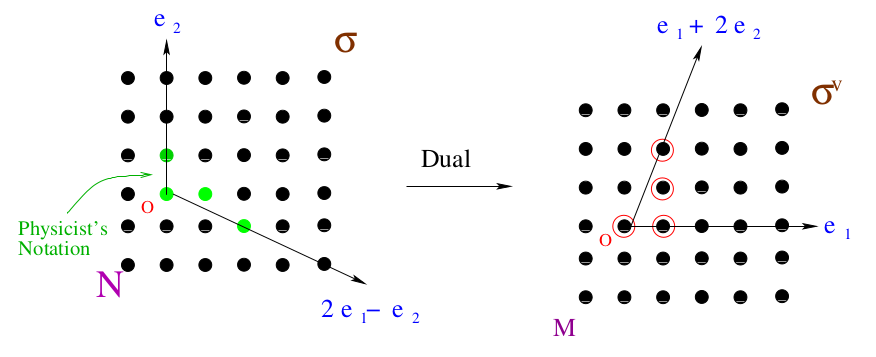
\includegraphics[scale=0.4]{Pictures/toricdiagZ2orbifold.png}
                \caption{Representations of the cone and dual cone in the lattice $\Z^2$.}
            \end{figure}

            The previous example illistrate a more genral result:
            \begin{prop*}
                All abelian orbifolds are toric varities.
            \end{prop*}
            Note that this result is not that surprising considering the general expression \eqref{eq:toricvargenform}.

            \begin{examp*}
                Let us start with $\sigma=\Cone(\{e_1,2e_1+e_2\})$. We then get $\sigma^\vee=\Cone(\{e_2,e_1-2e_2\})$ so $S_\sigma=\Span_{\Z^+}(\{e_2,e_1-2e_2\})$ and $\C[S_\sigma]=\C[y,xy^{-2}]=\C[u,v]$.
            \end{examp*}

            Now what happens with faces? An inclusion of face $\tau\subset\sigma$ gives an inclusions of the semigroups $S_\sigma\subset S_\tau$ and $\C[S_\sigma]\subset \C[S_\tau]$. This induces a morphism $U_\tau\to U_\sigma$ of affine toric varieties and it happens the this morphism is an open embedding.
            \begin{examp*}
                If $\sigma=\Cone(e_1,e_2)$ then we find $U_\sigma=\C^2$. There are three faces: $\rho_1=\Cone(e_1)$, $\rho_2=\Cone(e_2)$ and the origin $0$. These faces can be described by hyperplane $H_{e_2}, H_{e_1}$\todo{Why ?} and $H_{e_1+e_2}$ respectively, so we get
                \begin{align}
                    \C[S_{\rho_1}] &= \C[x,y,y^{-1}],
                    \C[S_{\rho_2}] &= \C[x,x^{-1},y],
                    \C[S_{0}] &= \C[x,y,x^{-1},y^{-1}].
                \end{align}
                They define the varieties $U_{\rho_1}=\C^*\times\C$, $U_{\rho_1}=\C\times\C^*$ and $(\C^*)^2$\todo{Why ?}, which are all open subvarieties of $\C^2$.
            \end{examp*}

        \subsection{Toric variety of a fan}
            
            A \emph{fan} is a collection $\Delta$ of cones in $N_\R$ such that each face of a cone is also a cone and the intersection of two cones is a face of each. Those two requirement imply in particular that the intersection of two cones in a fan is again a cone in the fan. Note that to any cone corresponds a fan containing the cone itself and all its faces.

            For a cone $\sigma$ in $N_\R$ the variety $U_\sigma$ contains the torus $T_N$ so fan in $N_\R$ produces a collection of varieties that all contain th same torus $T_N$. Gluing together the affine varities we obtain $X_\Delta$, it is clear that $T_N$ is an open subset of $X_\Delta$ and that $T_N$ acts on $X_\Delta$. This is called the \emph{toric variety of a fan}. For the toric varitey of a fan, each cone in the fan turns out to be determines an orbit $O(\sigma)$ of the torus.

            Generally speaking, an $m$-dimensional algebraic variety of a fan can be obtained as as particular holomorphic quotient of $\C^n$. If $\Z_\Delta\subset\C^n$ a set of points and $G\cong (\C^*)^{n-m}\times\Gamma$ is the group formed by the algebraic torus and an abelian discrete group $\Gamma$, then
            \begin{equation}
                \boxed{X_\Delta=\frac{\{\C^n\backslash\Z_\Delta\}}{G}.}\label{eq:toricvargenform}
            \end{equation}
            Let us explain this construction.
            
            If $\Delta$ is an $m$-dimensional fan, we denote by $\Delta(j)$ ($j\leq n$) the collection of $j$-dimensional cones in $\Delta$. The set $\Delta(1)\subset\Delta$ is then the collection of all one-dimensional cones in $\Delta$, i.e. the set of edges. To each cone $\sigma\in\Delta(1)$ is associated a unique vector $v_\sigma\in N$ that generates the sublattice $\sigma\cap N$. This vactor is called the \emph{primitive generator} of $\sigma$. Let $v_1,\dots,v_n$ be the primitive generators of of each $\sigma\in\Delta(1)$. Note that we always have $n\geq m$ since $\Delta$ is $m$-dimensional. Each vector $v_i$ has component $v^k_i$ ($i=1,\dots,n$,$k=1,\dots,m$) so we can construct an $m\times n$ matrix by putting the vectors in columns:
            \begin{equation}
                V=
                \begin{bmatrix}
                    v^1_1 & & & \cdots & \hspace{0.5cm} & & v^1_n \\
                    \vdots & & & & & & \vdots \\
                    v^m_1 & & & \cdots & & & v^m_n
                \end{bmatrix}
            \end{equation}
            This defines a linear map from $\C^n$ to $\C^m$ whose kernel is $\C^{n-m}$. Let $Q^a$ ($a=1,\dots,n-m$) be vectors that generate this kernel, then we must have
            \begin{equation}
                VQ^a=0\Leftrightarrow \sum^n_{i=1}v^k_i Q^a_i=0,\qquad k=1,\dots,m\label{eq:detQalpha}
            \end{equation}
            for all $a=1,\dots,n-m$. We now put that on the side for a moment. To each edge $\sigma\in\Delta(1)$ with associate a complex coordinate $x_\sigma$
            and consider the new map
            \begin{equation}
                \phi:\left(
                \begin{array}{ccc}
                    \C^n & \longrightarrow & \C^m \\
                    (z_1,\dots,z_n) & \longmapsto & (\prod^n_{i=1}z^{v^1_i}_i,\dots,\prod^n_{i=1}z^{v^m_i}_i)
                \end{array}
                \right).
            \end{equation}
            It is clear that the kernel of $\phi$ is $\tilde{G}\equiv\Ker(\phi)=(\C^*)^{n-m}$. \todo{Why ?} One can see that this kernel naturally acts on $\C^n$ as
            \begin{equation}
                \left(
                \begin{array}{ccc}
                    (\C^*)_a\times\C^n & \longrightarrow & \C^n \\
                    (\lambda,z_1,\dots,z_n) & \longmapsto & (\lambda^{Q^a_1} z_1,\dots,\lambda^{Q^a_n} z_n)
                \end{array}
                \right)
            \end{equation}
            where $Q^a_i$ are the component ofthe vectors $Q^a$ defined above. We defined the action of $\tilde{G}=(\C^*)^{n-m}$ on $\C^n$for each factor separately for simplicity.

            The $n$ vecotrs $v_i$ generate over $\Z$ a sublattice of $N$ that we denote $N'$. The discrete group obtained by taking the quotient of $N$ by this sublattice
            \begin{equation}
                \Gamma=N/N'
            \end{equation}
            is a subgroup of $G$ and taking the quotient by $\Gamma$ gives rise to the orbifold singularities.

            The last piece of data in the construction is the zero set $Z_\Delta$. Let us denote by $\mathcal{S}$ any subset of $\Delta(1)$ that does not generate a cone in $\Delta$ and $V(\mathcal{S})\subset\C^n$ the linear subspace defined by setting $x_\sigma=0$ for all $\sigma\in\mathcal{S}$, i.e. the hyperplane generated by the edges that does not generate a cone in $\Delta$. We the denote $Z_\Delta$ the union of all those hyerplanes, i.e. of all the $V(\mathcal{S})$. Our toric variety is defined as a qutient of $\C^n\backslash Z_\Delta$.

            To summarize, we can construct affine toric variety $X_\Delta$ from the $m$-fan $\Delta$ by following these steps:
            \begin{itemize}
                \item find the primitive generators $v_1,\dots,v_n$ of the $1$-cones of $\Delta$
                \item find the $n-m$ vectors $Q^a$ such that $\sum_iv^k_i Q^a_i=0$
                \item compute $\Gamma=N/N'$
                \item find the subsets of $\{v_1,\dots,v_n\}$ that don't generate in $\Delta$ and compute $Z_\Delta$
                \item the toric affine variety is $X_\Delta=(\C^n\backslash Z_\Delta)/((\C^*)^{n-m}\times\Gamma)$.
            \end{itemize}

            \begin{examp*}
                If we consider the $2$-dimensional fan $\Delta=\Fan(e_1,e_2,-e_1-e_2)$ in $N=\Z^3$ (so $m=2$), we have three one-dimensional cones generated by $v_1=e_1,v_2=e_2$ and $v_3=-e_2-e_2$ (so $n=3$) and the component matrix is
                \begin{equation}
                    \begin{bmatrix}
                        1 & 0 & -1 \\
                        0 & 1 & -1
                    \end{bmatrix}.
                \end{equation}
                We only have one vector $Q^a$ to find and since it must satisfy the relation \eqref{eq:detQalpha}, i.e. in this case $Q_1v_1+Q_2v_2+Q_3v_3=0$, it implies that $Q=(1,1,1)$. The group action of $\tilde{G}=\C^*$ on the $\C^3$ is then
                \begin{equation}
                    (z_1,z_2,z_3)\mapsto (\lambda z_1,\lambda z_2\lambda z_3).
                \end{equation}
                Since $v_1,v_2$ and $v_3$ generate all of $\Z^2$, $\Gamma=\{0\}$ is the trivial group and $G=\tilde{G}\times\Gamma\cong\cong\tilde{G}=\C^*$. There is no subset of $\{v_1,v_2,v_3\}$ that generates a cone which is not in $\Delta$ (because we defined $\Delta$ as the fan generated by those vectors in the first place) therefore $Z_\Delta=\{(0,0,0)\}$. \todo{Why?} Finally, the affine toric variety of $\Delta$ is
                \begin{equation}
                    X_\Delta=\frac{\C^3\backslash Z_\Delta}{G}=\frac{(\C^*)^3}{\C^*}=\C\P^2.
                \end{equation}
            \end{examp*}

            \begin{prop*}
                A toric variety $X_\Delta$ is compact if and only its fan $\Delta$ span the $N_\R$.
            \end{prop*}

        \subsubsection{Fan from a toric variety}

        \subsection{More general constructions}

            In general, an affine variety canbe defined by an ideal in $\C[x_1,\dots,x_n]$. In the same way, a toric affine variety can be defined by a \emph{toric ideal} (or \emph{binomial ideal}), i.e. an ideal in $\C[x_1,\dots,x_n]$ generated by binomials (polynoamils with precisely two non-zero coefficients).
            \begin{theorem*}
                Let $V$ be an affine variety. The following are equivalent:
                \begin{itemize}
                    \item $V$ is toric,
                    \item $V=\Spec(\C[S])$ for an affine semigroup $S$,
                    \item $V=V(I)$ for a toric ideal.
                \end{itemize}
            \end{theorem*}
            This is a very powerfull theorem since is states that an affine avariety is toric if and only if the generating polynomials of its ideal are binomials.

            %Toric varities of a cone are a way to construct toric varieties but there are others that we will not detail here.

    \subsection{Relation between fan varieties, cone varities and local coordinates}

        Given an $m$-dimensional cone spanned by $n$ vectors $v_1,\dots,v_n$, we want to find the local coordinates associated to it. Since the the toric variety can be expressend as the quotient by $G$, the local coordinates should $G$-invariant polynomials, that is polynomials $x=z^{n_1}_1\dots z^{n_n}_n$ such that
        \begin{equation}
            x\mapsto \lambda^{\sum_i Q^a_i n_i}x=x
        \end{equation}
        under $G$. But remember that \eqref{eq:detQalpha} so we can take $n_i=\langle w,v_i\rangle$ for any $w\in M$. We foud that the local coordinates are in one-to-one correspondence with the dual lattice $M$.    
    
        Given a fan and its fan toric variety, we can a toric affine variety to each top-dimensional cone. These cone toric varities will be affine patches of the fan variety. The transition functions between these patches are also encoded in the initial fan. Let us explain those statement in greater details. If $\sigma_i\in\Delta$ are the top-dimensional cones of a given fan $\Delta$, we can construct their toric variety $U_{\sigma_i}$ by following the procedure that we presented above. The toric varieties $U_{\sigma_i}$ act as affine pacthes and can be patched together to form $X_\Delta$. Now suppose that $\tau$ is a face of both $\sigma_i$ and $\sigma_j$, one can show that
        \begin{equation}
            \sigma^\vee_{i,j}\subset\tau^\vee\quad\Rightarrow\quad \C[\sigma^\vee_{i,j}\cap M]\subset\C[\tau^\vee\cap M]\quad\Rightarrow\quad U_\tau\subset U_{\sigma_i}\cap U_{\sigma_j}
        \end{equation}
        so the affine set associated to the fae $\tau$ is in the intser section of the affine sets of the cones. The relation between local coordinates $x^(i)$ of $U_{\sigma_i}$ and $x^(j)$ of $U_{\sigma_j}$ can then be read from the relations between the generators of $\sigma^\vee_{i,j}\cap M$ and $\sigma^\vee_{i,j}\cap M$:
        \begin{equation}
            \sum^{r_i}_{l=1}q_lw^{(i)}_l = \sum^{r_j}_{k=1}q_kw^{(j)}_k,\quad q_l,q_k\in\Z\quad\Rightarrow\quad \prod^{r_i}_{l=1}(x^{(i)}_l)^{q_l} = \prod^{r_j}_{k=1}(x^{(j)}_k)^{q_k}.\label{eq:chgtcoordtoric}
        \end{equation}
        We see that those transition functions are always rational functions. This is crucial property of toric varieties.

        \begin{examp*}
            Going back to the fan of $\C\P^2$, we see that there are three top-dimensional cones $\sigma_1,\sigma_2$ and $\sigma_3$. For each we have $U_{\sigma_i}=\C^2$. Applying \eqref{eq:chgtcoordtoric} we find that the transition functions between the cooridnates $(x_1,x_2)$ of $U_{\sigma_1}$ and $(y_1,y_2)$ of $U_{\sigma_2}$ are
            \begin{equation}
                x_1=\frac{y_1}{y_2},\quad x_2=\frac{1}{y_2}.
            \end{equation}
        \end{examp*}

    \subsection{Calabi-Yau toric varities}

        As motivated in the beginning, we are mainly interested in Calabi-You affine varities, so Calabi-Yau affine toric varieties in this case. A very convenient property of the toric varieties is that the CY condition is translated into a simple condition on the combinatoric data of the variety.

        Recall that a divisor of an affine variety is a linear combination of codimension-one irreducible subvarieties. A \emph{toric divisor} is a divisor invariant under the action of $G$. Using the homogeneous coordinates $(z_i)$, we can easily construct $G$-invariant subvarieties. The simple algebraic subsets
        \begin{equation}
            \{(z_1,\dots,z_n)|z_i=0 \forall i\in I\subset\{1,\dots,n\}\}
        \end{equation}
        are $G$-invariant so the subvarieties
        \begin{equation}
            D_i=\{z_i=0\}\cap X_\Delta
        \end{equation}
        are toric divisors. Even stronger, one can actually show that they generate the full group of divisors of $X_\Delta$ and that if $X_\Delta$ is smooth with canonical bundle $K_X$, we have
        \begin{equation}
            K_X=\mathcal{O}\left(-\sum^n_{i=1} D_i\right).
        \end{equation}
        This important result allows us us to state the Calabi-Yau condition (triviality of the canonical bundle) in a very simple way. The only thing left is to see that any $G$-invairant function is asection of the trivial bundle and that $K_X=\mathcal{O}\left(-\sum^n_{i=1} D_i\right)$ is trivial if and only if
        \begin{equation}
            G:z_1\dots z_n\mapsto\lambda^{\sum^n_{i=1}Q^a_i}z_1\dots z_n\quad\Leftrightarrow\sum^n_{i=1}Q^a_i=0.
        \end{equation}
        This last condition is equivalent to the existence of a vector $w\in M$ such that $\langle w,v_i\rangle=1$ for all $v_i$ in the fan. Finally, we get the follwing criteria:
        \begin{prop*}
            The toric variety $X_\Delta$ is CY if and only if all the vectors $v_i$ in $\Delta$ end on the same hyperplane in $N$, which happens if and only if $\sum^n_{i=1}Q^a_i=0$ for $a=1,\dots,n-m$.
        \end{prop*}

        Following from the proposition on compactness of toric varieties that we gave before, this implies tha toric CY varieties are necessarily non-compact.

        \begin{table}[H]
            \centering
            $
            \begin{array}{|c|c|c|c|c|c|}
                \hline
                X_\Delta & \dim_\C & \text{generating polynomial} & \text{compact} & \text{CY} & \Delta \\ \hline
                \C^2 & 2 & & \text{no} & \text{yes} & \Fan(e_1,e_2) \\ \hline
                \C^2/\Z_k & 2 & uv-w^2 & \text{no} & \text{yes} & \Fan(e_2,ke_1-e_2) \\ \hline
                \C^3/\Z_k & 3 &  & \text{no} & \text{yes} & \Fan(e_2,ke_1-e_2,e_3) \\ \hline
                \mathcal{C}_0 & 3 & x_1x_2-x_3x_4 & \text{no} & \text{yes} & \Fan(e_3,e_1+e_3,e_1+e_2+e_3,e_2+e_3) \\ \hline
                \text{SSP} & & & & & \\ \hline
            \end{array}
            $
            \caption{Useful list of toric varieties.}
        \end{table}

    \subsection{Toric diagrams and p-q webs}

        For CY toric varieties, the combinatoric information encoded in the fan can be expressed in term of a reduced lattice of one less dimension. This is espacially convenient for us since we are mainly concerned about toric CY threefolds, which can therefore be fully encoded in the $2$-dimensional lattice. Indeand, instead of drawing a $3$-dimensional fan, we can simply project iton the special plane defined by $\langle w,v_i\rangle=1$, and we get the \emph{toric diagram}.

        We can also write the dual of the toric diagram by replacing each line with an orthogonal line. This is called the \emph{peq-web}. They have a nice physical interpreatation as webs intersecting $5$-banes.

    \subsection{Singularities}

        A cone is said to be \emph{smooth} if it is generated by part of a lattice basis.
        \begin{theorem*}
            A cone $\sigma$ is smooth of and only if $U_\sigma$ is smooth.
        \end{theorem*}
        \begin{examp*}
            The affine toric variety $Z(x^2-y^3)$ discuss above is not smooth.
        \end{examp*}

        \begin{prop*}
            The varitey $X_\Delta$ is is non-singular if and only if $\Delta$ is a smooth fan.
        \end{prop*}


        A toric variety is nonsingular if its cones of maximal dimension are generated by a basis of the lattice. This implies that every toric variety has a resolution of singularities given by another toric variety, which can be constructed by subdividing the maximal cones into cones of non-singular toric varieties.

\section{Important examples}
    
    \subsection{The conifold}

        The singular conifold $\mathcal{C}_0$ can be viewed as the toric variety of the fan $\Delta=\Fan(e_3,e_1+e_3,e_1+e_2+e_3,e_2+e_3)$ in $\Z^3$. This fan contains $10$ cones on total. Denoting the four generating vectors as $v_1,v_2,v_3$ and $v_4$, we find that the only charge vector $Q$ must satisfy $Q_1v_1+Q_2v_2+Q_3v_3+Q_4v_4=0$ which gives $Q=(1,-1,1-1)$ so $\tilde{G}=\C^*$ acts as
        \begin{equation}
            (z_1,z_2,z_3,z_4)\mapsto (\lambda z_1,\lambda^{-1} z_2\lambda z_3,\lambda^{-1} z_4).
        \end{equation}
        We also find that $\Gamma=\{0\}$ is the trivial group and that $Z_\Delta=Z(z_1,z_3)\cup Z(z_2,z_4)$. Finally,
        \begin{equation}
            \mathcal{C}_0=\frac{\C^3\backslash Z_\Delta}{\C^*}.
        \end{equation}

        Note that, by definition we also have $\mathcal{C}_0=Z(x_1x_4-x_2x_3)$ so it is generated by a binomial andistherefore expected to be toric. 

        \begin{figure}[H]
            \centering
            \begin{subfigure}[b]{0.3\textwidth}
                \centering
                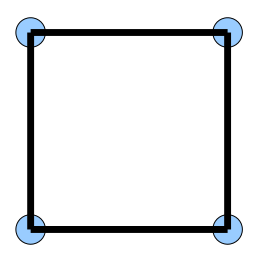
\includegraphics[scale=0.4]{Pictures/conifoldtoricdiag.png}
                %\caption{Toric digram of the conifold.}
                \label{fig:y equals x}
            \end{subfigure}
            \hspace{2cm}
            \begin{subfigure}[b]{0.3\textwidth}
                \centering
                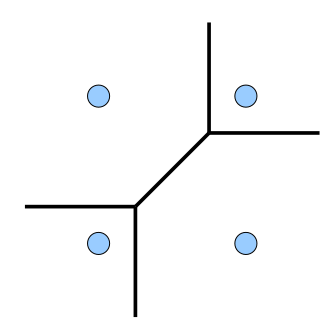
\includegraphics[scale=0.3]{Pictures/conifoldpqweb.png}
                %\caption{pq-web of the conifold.}
                \label{fig:three sin x}
            \end{subfigure}
            \caption{Toric diagram and pq-web of the conifold.}
            \label{fig:Z5graphs}
       \end{figure}

    \subsection{The suspended pinch point}

       \begin{figure}
           \centering
           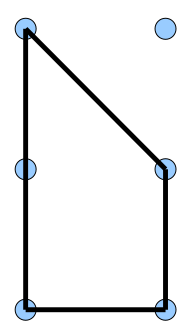
\includegraphics[scale=0.4]{Pictures/SPPtoricdiagram.png}
           \caption{Toric diagram of the SPP.}
       \end{figure}

    \subsection{del Pezzo surfaces}

\section{Gauged linear sigma model (GLSM)}

    Witten's gauged linear sigma model provides a physical perspective on toric varieties which provides us with the right approach for the forward algorithm. Let us consider the vectorspace $\C^q$ with complex coordinates $z_1,\dots,z_q$.
        

    \subsection{Calabi-Yau and non-compactness conditions}

\section{Correspondence between gauge theory and singularity}

    Above, we presented all the possible orbifold constructions of supersymmetric quiver gauge theories in four dimensions. We started from quotienting the transverse space and we found the corresponding (supersymmetric) gauge theory. In other words, we started from the singularity a found the gauge theory. We can therefore consider that the orbifold singularities are understood. However, not all singularities are orbifold one, such as the conifold for example. We can then ask ourselves how to obtain the gauge theory for more general singularities than the orbifold ones. Is a general approach possible ? On the other hand, we can also study the converse question; is it possible to to obtain the singularity from the gauge theory? And if it is, how so? In general we will see that there is a bijection between the four-dimensional supersymmetric worldvolume gauge theory and the Calabi-Yau singularity. We now detail this bijection.

    \begin{figure}[H]
        \centering
        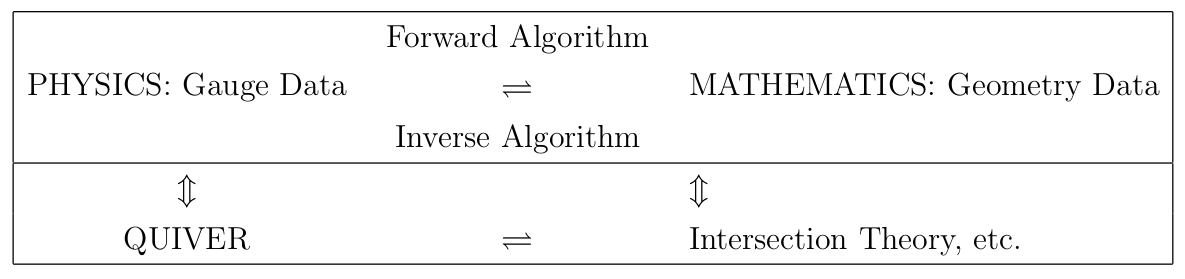
\includegraphics[scale=0.3]{Pictures/algorithm.png}
        \caption{Inverse and forward algorithm, from \cite{he2004lectures}.}
    \end{figure}

    \subsection{From gauge theory to singularity: forward algorithm}

        We start with the simplest question: how to recover the singularity from the gauge theory? We already mentioned that the vacuum parameter space of the scalar fields of the gauge theory is the so-called moduli space, denoted $\M$. Because our D$3$-brane is a point in the Calabi-Yau threefold, the vacuum moduli space $\M$ is the affine coordinates of the Calabi-Yau singularity $S$.

        For the ADE $\mN=2$ theories discussed in section \ref{sec:N2QGT}, by the Kronheimer-Nakajima construction \cite{Kronheimer1990}, the moduli space is a hyper-Kähler quotient. In general, the moduli space can be constructed as a \emph{quiver variety}, i.e. a variety constructed from the moduli space of quiver a quiver representation. More rpecisely, given the dimensions of the vector spaces assigned to every vertex, one can form a variety which characterizes all representations of that quiver with those specified dimensions, and consider stability conditions. Let us see some examples of this.

        The anomaly free condition is
        \begin{equation}
            (a_{ij}-a_{ji})n_i=0.
        \end{equation}
        \todo{Explain more.}

    \subsection{Forward algorithm for abelina orbifolds}

        

    \subsection{From singularity to gauge theory: inverse algorithm}

        Mathematically, a quiver gauge theory is a representation of a finite quiver with relations. The labels are $\{N_i\in\Z_+\}$, they correspond to the dimension of the vector space $\{V_i\}$. The gauge group is $\prod_i\SU(N_i)$. The gauge fields are self-adjoint arrows $\Hom(V_i,V_i)$ while the matter fields are bi-fundamentals fermions/bosons and are arrows $X_{ij}\in\Hom(V_j,V_i)$. For a quiver with adjacency matrix $a_{ij}$, the gauge anomaly cancellation condition can be generally expressed as
        \begin{equation}
            (a_{ij}-a_{ji})N_i=0.
        \end{equation}
        At last, there are some relations that arises the superpotential $W(\{X_{ij}\})$. The vacuum is the minima of the superpotential. In other words,
        \begin{equation}
            \pdv{W}{X_{ij}}=0.
        \end{equation}

    \subsection{Application to Toric del Pezzo's}

        \begin{figure}
            \centering
            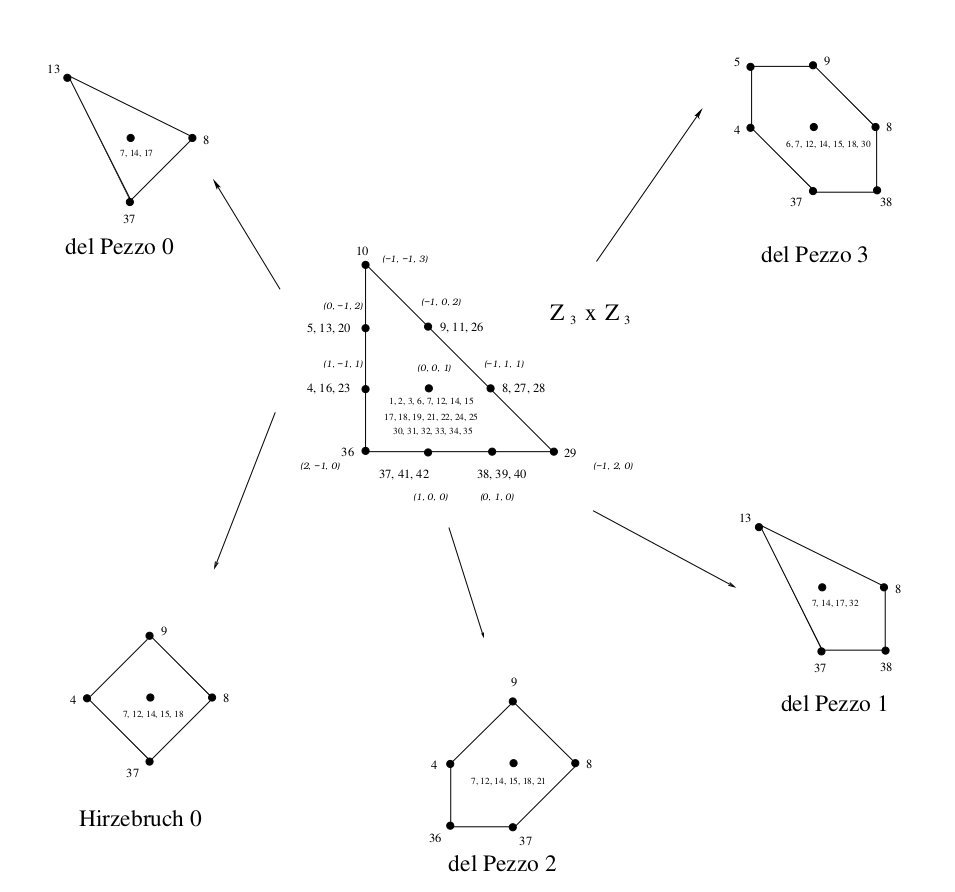
\includegraphics[scale=0.4]{Pictures/delPezzo.png}
        \end{figure}

\section{Toric duality}

